\documentclass[12pt]{article}
\usepackage[margin=0.75in,tmargin=1in]{geometry}
\usepackage{fancyhdr}
\usepackage{amsmath}
\usepackage{graphicx}
\graphicspath{ {./images/} }

\title{MATH 3012: Applied Combinatorics}
\author{Jaeheon Shim}
\date{}

\begin{document}

\pagestyle{fancy}
\fancyhead[L]{MATH 3012: Applied Combinatorics}

\maketitle
\thispagestyle{fancy}

\section{Sets}
The first order of business is a review of basic set principles and notation.
\subsection{Sets}

A set is a collection of objects. Below are two examples of sets:
\begin{align*}
	A &= \{1, 2, 3\} \\
	B &= \{A, -2.7, ARTICHOKE\}
\end{align*}
\begin{itemize}
	\item The order of elements does not matter
	\item Repeated elements are not allowed
\end{itemize}
The $\emptyset$ symbol denotes the empty set. The empty set is the set containing no elements.\\\\
Below are some symbols related to sets.
\begin{itemize}
	\item
		$\mathbf{b \in A}$ - element $b$ is a member of set $A$ \\
		$$1 \in \{1, 2, 3\}$$
		$$7 \not\in \{1, 2, 3\}$$
		$$\emptyset \in \{1, 2, 3\}$$
	\item
		$\mathbf{A \subseteq B}$ - A is a subset of B (Every element of A is also in B)
	\item
		$\mathbf{A \not\subseteq B}$ - A is not a subset of B (There exists an element of A that is not in B
	\item
		$\mathbf{\exists}$ - "there exists" \\
		$$\exists x \in \{7, 8\} \text{ such that } x > 5$$
	\item
		$\mathbf{\forall}$ - "for all" \\
		$$\forall x \in \{7, 8, 9\}, x \geq 4$$
	\item
		$\mathbf{B = \{x \in A \mid x > 4\}}$ - An example of set builder notation. "The set containing every element in A that is greater than 4"
	\item
		$\mathbf{\cup}$ - Set Union: Elements in either set or both\\
		$$ \{1, 2, 3, 4\} \cup \{3, 4, 5, 6\} = \{1, 2, 3, 4, 5, 6\} $$
	\item
		$\mathbf{\cap}$ - Set Intersection: Elements in both sets\\
		$$ \{1, 2, 3, 4\} \cap \{3, 4, 5, 6\} = \{3, 4\} $$
	\item
		$\mathbf{|A|}$ - Cardinality: The size of a set\\
		$$ A = \{1, 2, 3, 4\} \qquad |A| = 4$$
\end{itemize}

	\subsection{The Cartesian Product}
	The cartesian product is an operation that can be applied to two sets.\\\\
	\textbf{Example}\\
	Let $A = \{1, 2\},\quad B = \{3, 4\}$
	\begin{align*}
		A \times B &= \{(x, y) \mid x \in A, y \in B\} \\
		&= \{(1, 3), (1, 4), (2, 3), (2, 4)\} 
	\end{align*}

	More formally,
	$$ A_1 \times A_2 \times \cdots \times A_n = \{(a_1, a_2, \ldots, a_n) \mid a_i \in A_i \forall i \in {1, 2, \ldots, n} \} $$

	Notice the elements of the set produced by the cartesian product are contained in parentheses '()' instead of curly brackets '\{\}'. This denotes that they are a tuple. In a tiple, \textbf{order matters} and \textbf{repeates are allowed}.\\\\
	\textbf{The Product Rule} \\ 
	$$|A \times B| = |A| \cdot |B|$$

	\section{Counting}
	\subsection{Fundamental Principles of Counting}
	\subsubsection{Rule of Sum}
	If there are $m$ possible choices for a task, and $n$ possible choices for another task, performing either task can be completed in one of $m + n$ ways. \\\\
	\textbf{Example}\\
	You can choose either sprinkles or syrup \textbf{but not both} as topping for your ice cream. There are 4 kinds of sprinkles and 3 kinds of syrup. Therefore, there are $4 + 3 = 7$ total different ways to choose a topping for your ice cream.
	\subsubsection{Rule of Product}
	If a choice has two stages with $m$ possibilities in the first stage and $n$ possibilities in the second stage, there are $(m)(n)$ total possibilities.\\\\
	\textbf{Example}\\
	You are at a restauraunt in Paris about to enjoy a three course meal. There are 3 choices for the appetizer, 4 choices for the main course, and 2 choices for dessert. Therefore, there are $(3)(4)(2) = 24$ different three course meals you are able to enjoy. 
	\subsection{Permutations}
	Permutations refer to the counting of possible rearrangements of some number of objects, assuming each object is distinguishable. \\\\
	Suppose we have 10 differently colored blocks, and we want to find out how many ordered arrangements of 4 blocks we can form.\\\\
	We can think of choosing each block in stages using the rule of product. We have 10 choices for the first block, 9 choices for the second, 8 for the third, and 7 for the fourth. Therefore, there are $10 * 9 * 8 * 7 = 5040$ possibilities.
	\begin{align*}
		10 * 9 * 8 * 7 &= \frac{10 * 9 * 8 * 7 * 6 * 5 * 4 * 3 * 2 * 1}{6 * 5 * 4 * 3 * 2 * 1} \\
		&= \frac{10!}{6!} \\
		&= \frac{10!}{(10 - 4)!}
	\end{align*}
	From this, we can derive a general formula for permutations. $n$ refers to the number of total objects, and $r$ refers to the number of objects we want to form a permutation with.
	$$P(n, r) = \frac{n!}{(n - r)!}$$
	\textbf{Example}\\
	How many ways are there to rearrange the word DATABASES into distinct strings? \\\\
	We can apply our logic of having 9 choices for the first letter, 8 for the second, ... However, this will \textit{overcount} certain strings, as there exist duplicates letters in the string. Therefore, we need to divide to correct for overcounting. \\\\
	There are 2 S's in DATABASES, the position of which can be flipped in the rearranged string. Therefore, we must divide by 2. Similarly, there are 3 A's, of which there are $3! = 6$ rearrangements. The number of distinct rearrangements we can create is
	$$\frac{9!}{3!2!} = 30240$$
	\subsection{Strings}
	Let $X$ be a set. A string over the \textit{alphabet} $X$ is a sequence of elements of X (order matters).\\\\
	\textbf{Example}\\
	Consider a set Y
	$$ Y = \{a, b, \ldots, z\} $$
	The following are examples of strings over Y
	\begin{itemize}
		\item (a, b, c, d, e)
		\item (h, e, l, l, o)
	\end{itemize}
	\textbf{Example}\\
	How many strings of length 6 are there over the alphabet $L = \{a, b, \ldots, z\}$ \textbf{with no repeated characters}? \\\\
	26 options for postion 1, 25 for position 2, 24 for position 3, ...
	$$(26)(25)(24)(23)(22)(21)$$
	More generally, let X be a set with $|X| = n$ and let $k \in \mathbf{N}$ with $k \leq n$ \\
	The number of strings of length k over X with no repeated characters is
	\begin{align*}
		(n)(n - 1)(n - 2)\cdots(n - k + 1) = \frac{n!}{(n - k)!}
	\end{align*}
	\subsection{Combinations}
	Suppose we have 10 differently colored blocks, and we want to find out how many different sets of 4 blocks we can choose from the set of 10 (order doesn't matter).\\\\
	We could start out by listing out the number of possible combinations.
	$$ \frac{10!}{(10 - 4)!} $$
	However, this formula would count each of the following arrangements of blocks (for example) even though they all contain the same 4 colors.
	\begin{align*}
		\{R, B,& O, G\}\\
		\{B, R,& G, O\}\\
		\{G, O,& R, B\}\\
		\{O, R,& B, G\}\\
			   &\vdots
	\end{align*}
	We need to correct for overcounting. Notice that there will be $4!$ different ordered arrangements of these same 4 colors. Let's update our formula.
	$$\frac{10!}{(10 - 4)!4!}$$
	We divide by $4!$ to account for overcounting, and our formula is now correct.\\\\
	More generally, there are $$\frac{n!}{(n - k)!k!}$$ ways of choosing a set of k elements from a set of n elements. There exists a special notation for this formula:
	$${n \choose k} = \frac{n!}{(n - k)! k!}$$
	\textbf{Example}\\
	How many license plates are there with 6 characters over the alphabet $\{A, \ldots, Z, 0, \ldots, 9\}$ where exactly two characters are numbers and exactly one is a vowel?\\\\
	There are ${6 \choose 2}$ ways of choosing which two positions are numbers, and after two positions are chosen ${4 \choose 1}$ ways to choose which character is a vowel. There are $10*10$ ways to choose the two numbers, $5$ ways to choose the one vowel, and $21$ ways to choose the remaining 3 consonants.
	$${6 \choose 2}{4 \choose 1}(10^2)(5)(21^3)$$
	\textbf{Property}\\
	${n \choose k} = {n \choose n - k}$\\\\
	\textbf{Algebraic Proof}
	\begin{align*}
		{n \choose k} &= \frac{n!}{(n - k)!k!}\\
					  &= \frac{n!}{(n-k)!(n - (n - k))!}\\
					  &= {n \choose n - k}
	\end{align*}
	\textbf{Combinatorial Proof}\text{ (More on this later)}\\
	Suppose we have a club of n people, and we need to choose a team of k people from that club to participate in a competition. How many ways are there to do this? We can either:
	\begin{enumerate}
		\item Choose k people from n people ${n \choose k}$
		\item Choose the $(n - k)$ people who will not make the team ${n \choose n - k}$
	\end{enumerate}
	\subsection{Combinatorial Proofs}
	We can show that some equation holds by showing that the LHS (Left Hand Side) and RHS (Right Hand Side) are just two different ways of counting the same thing.\\\\
	\textbf{Example}\\
	If $n = 2k$, where k is a natural number, $2^k \vert n!$ ($2^k$ evenly divides $n!$).\\\\
	\textbf{Proof}\\
	Say you have $n$ symbols where there are pairs of interchangeable elements.
	$$x_1, x_1, x_2, x_2, \ldots x_{n-1}, x_n$$
	There are $n!$ ways to arrange these symbols, including $2^k$ for every interchangeable pair of elements. Therefore, the number of unique arrangements is equal to 
	$$\frac{n!}{2^k}$$
	Since we can apply this method to reduce overcounting, $n!$ is divisible by $2^k$
	\subsection{Stars and Bars}
	So far, we've seen counting problems where in order to count something we've had to repeatedly answer the question "how many options are there for what goes here?"\\\\
	The next counting technique can be best illustrated with an example.\\\\
	\textbf{Example}\\
	In how many ways can I distribute 10 \textbf{identical} flowers between Sarah, Erin, and Paul?\\\\
	We can model our solution as a string over the alphabet $\{\star, \vert\}$ with exactly 10 $\star$'s (representing the 10 flowers and \textbf{2} $\vert$'s, which will divide our 10 flowers into 3 portions. Below is an example of a string describing one scenario in which this can happen:
	$$\{\star, \star, \star, \vert, \star, \star, \vert, \star, \star, \star, \star, \star\}$$
	\begin{center}
		\textit{Sarah gets 3 flowers, Erin gets 2, and Paul gets 5.}
	\end{center}
	The question thus becomes, how many strings of length 12 are there over $\{\star, \vert\}$ with exactly 2 $\vert$s? We can choose the locations to place the $\vert$s:
	$${12 \choose 2}$$
	\textbf{Generally,} there are ${n + m - 1 \choose m - 1}$ ways of sharing n identical objects among m people.\\\\
	\textbf{Variations}\\
	We can be a bit more abstract and use variables instead of characters in a story.
	$$x_1 + x_2 + x_3 + x_4 = n$$
	\begin{center}
		\textit{How many ways are there to distribute n objects among the variables $x_1, x_2, x_3, x_4$?}
	\end{center}
	There are also variations on this method:
	\begin{itemize}
		\item $x_1 + x_2 + x_3 + x_4 = n$ such that $x_1 \geq 2$ \\
			$x_1$ must be at least 2, so we set aside 2 for $x_1$ at the beginning, then run stars and bars on the remainder. ${n - 2 + 3 \choose 3}$
		\item $x_1 + x_2 + x_3 + x_4 \leq n$ \\
			Imagine adding another variable that can 'absorb' 0 to n elements. Then, $x_1 + x_2 + x_3 + x_4$ are left with the elements that were not absorbed (n to 0). This accounts for the constraint $\leq n$, as now each case for n is considered. \\
			In essence, rewrite as $x_1 + x_2 + x_3 + x_4 + x_5 = n$ and run stars and bars. ${n + 4 \choose 4}$
	\end{itemize}
	\noindent
	\subsection{Binomial Coefficients}
	Earlier, we introduced numbers of the form ${n \choose k} = \frac{n!}{(n - k)!k!}$. These numbers are caled "binomial coefficients". Here, we'll see why.
	\subsubsection{The Binomial Theorem}
	If $x, y$ are variables and $n$ is a positive integer, then
	\begin{align*}
		(x + y)^n &= {n \choose 0}x^0y^n + {n \choose 1}x^1y^{n-1} + {n \choose 2}x^2y^{n-2} \\
				  &= \ldots + {n \choose n}x^ny^0 \\
				  &= \sum_{k=0}^{n} {n \choose k}x^ky^{n-k}
	\end{align*}
	These numbers appear as the coefficients of this binomial.\\\\
	\textbf{Proof}\\
	Note that $(x + y)^n = (x+y)(x+y)\ldots(x+y)$ \\\\
	For each value of k with $k \in \mathbf{N}$ and $k \leq n$, the simplified expansion of the above product will have a term of the form $c \cdot x^ky^{n-k}$ where c is some constant corresonding to the number of times $x^ky^{n-k}$ appears.\\\\
	The term $x^ky^{n - k}$ appears once for every possible way to choose k x's from our n factors (and thus $n - k$ y's from our n factors).\\\\
	\textbf{Example}\\
	I'm labeling the variables with subscripts so it's more clear how they're distributed when the expansion is performed. There's otherwise nothing special about $x_A$, $x_B$ or $x_C$
	\begin{align*}
		(x+y)^3 &= (x_A+y_A)(x_B+y_B)(x_C+y_C) \\
				&= (x_Ax_B + x_By_A + x_Ay_B + y_Ay_B)(x_C+y_C) \\
				&= x_Ax_Bx_C + x_By_Ax_C + x_Ay_Bx_C + y_Ay_Bx_C + x_Ax_By_C + y_Ax_By_C + x_Ay_By_C + y_Ay_By_C
	\end{align*}

	Note that the term $xxy$ appears 3 times, once for every way in which we can choose x from two of the factors above. The two x's can be $x_Ax_B$, $x_Bx_C$, or $x_Ax_C$. \\\\
	\textbf{Example}\\
	What is the coefficient of $x^5y^2$ in the expansion of $(x + y)^2$?\\\\
	The coefficient for $x^kx^{7-k}$ is ${7 \choose k}$. Therefore, the coefficient for $x^{5}y^{7-5}$ is ${7 \choose 5}$.\\\\
	\textbf{Example}\\
	What is the coefficient of $a^6b^2$ in the expansion of $(7a-3b)^8$\\\\
	The binomial coefficient will be ${8 \choose 6}$. Don't forget to count $7^6$ and $(-3)^2$ too. The final answer is ${8 \choose 6}7^63^2$. \\\\
	This is useful because polynomials can be crafted in such a way that their coefficients are the answers to counting problems. These are called generating functions.

	\subsubsection{The Multinomial Theorem, a generalization of the Binomial Theorem}
	Let $n, t$ be positive integers and let $n_1, n_2, \ldots, n_t$ be natural numbers with $n_1 + n_2 + \cdots + n_t = n$. The coefficient of $x_1^{n_1}x_2^{n_2} \cdots x_t^{n_t}$ in the expansion of $(x_1 + x_2 + \cdots + x_t)^n$ is $\frac{n!}{n_1!n_2!\cdots n_t!}$ \\\\
	When $t = 2$, we recover the binomial theorem
	\begin{align*}
		n_1 + n_2 &= n \\
		n_2 &= n - n_1 \\
		\frac{n!}{n_1!(n - n_1)!} &= {n \choose n_1}
	\end{align*} 
	\textbf{Proof} 
	The proof is very similar to that of the binomial theorem. For $x_1^{n_1}x_2^{n_2} \cdots x_t^{n_t}$, we want the ways in which we can choose which $n_1$ of the $n$ factors contribute $x_1$ to the term, which $n_2$ of the \textbf{remaining} $n - n_1$ factors contribute $x_2$, ... etc.
	$${n \choose n_1}{n - n_1 \choose n_2}\cdots {n - n_1 - \ldots - n_{t-1} \choose n_t} = \frac{n!}{n_1!n_2!\cdots n_t!}$$
	\textbf{Notation}
	Numbers of this form are called multinomial coefficients
	$${n \choose n_1, n_2, \cdots, n_t} = \frac{n!}{n_1!n_2!\cdots n_t!}$$
	\section{The Principle of Mathematical Induction}
	Let P(n) be a statement involving some natural number, n.\\\\
	If:
	\begin{enumerate}
		\item P(0) is true
		\item For every $k \geq 0$, the truth of $P(k)$ implies the truth of $P(k + 1)$, then $P(n)$ is true $\forall n \in \mathbf{N}$
	\end{enumerate}
	\begin{align*}
		&P(0) \rightarrow P(1) \\
		&P(1) \rightarrow P(2) \\
		&P(2) \rightarrow P(3) \\
		&\ldots etc
	\end{align*}
	\subsection{The Well-Ordering Principle}
	\textbf{Induction CANNOT be used to prove things about subets of $\mathbf{R}$}. To use induction to prove statements, the first thing we need to do is prove our statement holds for the smallest element in the set. Not every subset of $\mathbf{R}$ has a smallest element.\\\\
	The reason we are able to use induction for $\mathbf{N}$ is due to the \textbf{Well-Ordering Principle}. The well-ordering principle states that every nonempty subset of $\mathbf{N}$ has a smallest element.
	\subsection{Proof of the Principle of Mathematical Induction}
	Complete Later
	\subsection{Prove that $\forall n \geq 1, \sum_{j = 1}^n j = \frac{n(n + 1)}{2}$}
	We proceed by induction on n. \\\\
	Note that when $n = 1$
	\begin{align*}
		\sum_{j = 1}^{1} j &= 1 \\
						   &= \frac{1(1 + 1)}{2} \\
	\end{align*}
	Let $k \geq 1$, and suppose the statement holds when $n = k$. \\\\
	Let $n = k + 1$
	\begin{align*}
		\sum_{j = 1}^{n} j &= \sum_{j = 1}^{k + 1} j \\
						   &= \left(\sum_{j = 1}^{k} j \right) + (k + 1) \\
						   &= \frac{k(k + 1)}{2} + (k + 1) \\
						   &= \frac{k(k + 1) + 2(k + 1)}{2} \\
						   &= \frac{(k + 1)((k + 1) + 1)}{2}, \text{as desired.}
	\end{align*}
	\subsection{Prove that $\forall n \geq 1$  $(n \in \mathbf{N})$, $\sum_{j = 1}^{n} (2j - 1) = n^2$}
	We proceed by induction on n.\\\\
	Note that when $n = 1$
	\begin{align*}
		\sum_{j = 1}^{1} (2j - 1) = 1
	\end{align*}
	Let $k \geq 1$, and suppose the statement holds when $n = k$. \\
	Let $n = k + 1 $
	\begin{align*}
		\sum_{j = 1}^{n} (2j - 1) &= \sum_{j = 1}^{k + 1} (2j - 1) \\
						   &= \left(\sum_{j = 1}^{k} (2j - 1)\right) + (2(k + 1) - 1)\\
						   &= k^2 + 2(k + 1) - 1 \\
						   &= k^2 + 2k + 2 - 1 \\
						   &= k^2 + 2k + 1 \\
						   &= (k + 1)^2,\quad \text{as desired.}
	\end{align*}
	\subsection{How to write a proof by induction}
	Say we want to prove a statement $P(n)$ holds for all $n \in \mathbf{N}$ with $n \geq b$. (Typically, $b \in \{0, 1\}$; it's usually the smallest number for which $P(n)$ makes sense.) \\\\
	Step 1: Establish a base case: prove that $P(b)$ is true. \\
	Step 2: State the inductive hypothesis.

	\textit{Suppose now $P(k)$ is true for some $k \geq b$.} \\
	Step 3: Perform the inductive step (i.e. show that $P(k) \rightarrow P(k + 1)$
	\section{Recursion}
	\textbf{Definition}\\
	A sequence of numbers $a_0, a_1, a_2, \ldots$ is recursive if the terms in the sequence are defined using previous terms in the sequence. \\
	The first few terms, which are not defined using the previous terms, are called the initial conditions\\\\
	\textbf{Example}\\
	\begin{align*}
		b_0 &= 1 \\
		b_n &= 2b_{n - 1} \forall n \geq 1
	\end{align*}
	$$b_0 = 1, b_1 = 2, b_2 = 4, \ldots $$
	\subsection{Recursion and Counting}
	Recursive relations can be used as solutions whose terms are the answers to counting problems. \\\\
	\textbf{Example}\\
	Let $n \in \mathbf{N}$, and suppose n (straight) lines are drawn in the plane so that
	\begin{enumerate}
		\item Every pair of lines crosses
		\item No three lines cross at a single point.
	\end{enumerate}
	Let $r_n$ denote the number of regions the plane is divided into by these lines. \\
	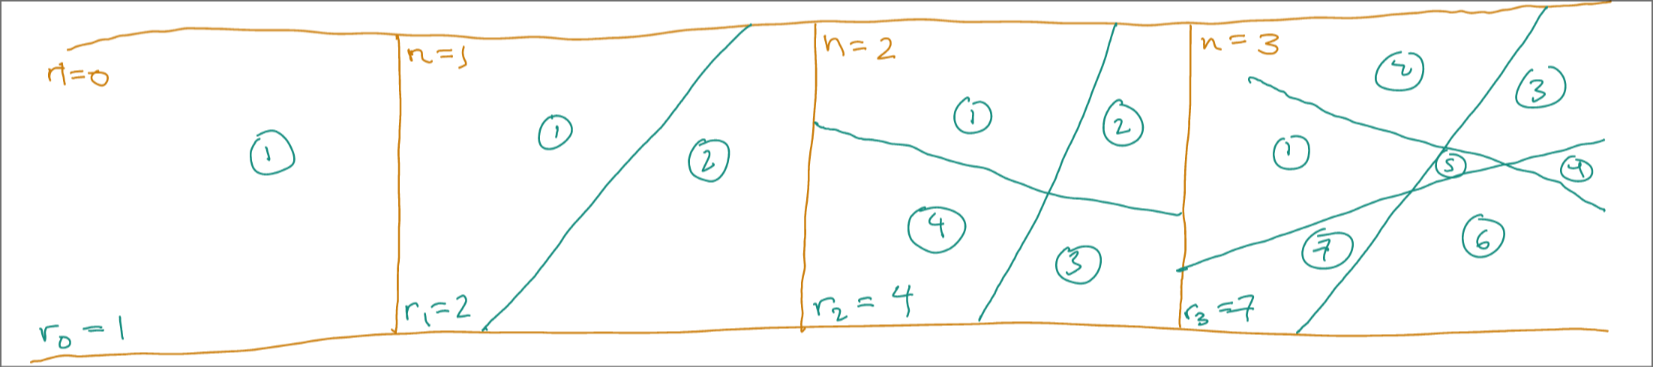
\includegraphics[scale=0.3]{recursion_counting1}\\
	\textbf{Solution}\\
	Suppose we have n lines drawn in the plane (where $n \geq 1$). Focus on one of the lines, L. Notice that L crosses every one of the remaining $n - 1$ lines exactly once, which divides L into exactly $n$ line segments.
	If we delete L, we have $r_{n - 1}$ regions. \textbf{Each of the n line segments that forms L divides on of these existing regions into two regions}. \\\\
	It follows that $r_n = r_{n - 1} + n \quad \forall n \geq 1$ and $r_0 = 1$ \\
	\noindent\rule{\textwidth}{1pt}
	\textbf{Example}\\
	We'll call a string over the alphabet $\{0, 1, 2\}$ "good" if it doesn't contain the substring "20" (otherwise we'll say it's "bad"). For all $n \in \mathbf{N}$, let $g_n$ be the number of good strings of length n. Find the recurrence relation and initial conditions for the sequence $g_0, g_1, g_2, \ldots$.\\\\
	\textbf{Solution}\\
	Take a good strin of length n, say $s_1s_2\ldots s_n$ \\\\
	Case 1. The last character $s_n$ is a 1. In this case, note that $s_1s_2\ldots s_{n - 1}$ can be any good string of length $n - 1$. In this case, $s_1s_2\ldots s_{n - 1}$ can be any good string of length $n-1$. There are $g_{n-1}$ of these.\\
	Case 2. Same as case 1 ("20" cannot be formed at the end) \\
	Case 3. $s_n = 0$ In this case, $s_{n-1}$ cannot be a 2. $s_1s_2 \ldots s_{n-1}$ can be any good string of length $n-1$ that doesn't end in 2.

	By case 2, there are $g_{n-2}$ good strings of length $n-1$ that end in a 2, and of course there are $g_{n - 1}$ good strings of length $n - 1$. So, there are $g_{n-1} - g_{n-2}$ good strings of length $n-1$ that don't end in a 2.\\\\
	Sum all of the cases:
	\begin{align*}
		g_n &= g_{n - 1} + g_{n - 1} + (g_{n - 1} - g_{n - 2}) \\
			&= 3g_{n - 1} - g_{n - 2} \forall n \geq 2
	\end{align*}
	Initial conditions:
	\begin{align*}
		s_0 &= 1 \quad \text{The empty string} \\
		s_1 &= 3 \quad \text{0, 1, \& 2}
	\end{align*}
	\section{The Pigeonhole Principle}
	If you have $n + 1$ objects, each of which needs to be put into one of $n$ categories, then at least one of the categories will contain at least 2 objects. \\\\
	A function $f: X \rightarrow Y$ is injective (or 1-to-1) if $\forall x_1, x_2 \in X$, $f(x_1) = f(x_2) \rightarrow x_1 = x_2$. That is, if $f(x_1)$ and $f(x_2)$ map to the same output, their inputs are also the same (i.e. no two distinct inputs get mapped to the same output)
\end{document}
env
